\documentclass{article}
\usepackage{polyglossia}
\usepackage{graphicx}
\usepackage[a4paper, portrait, margin=1in]{geometry}
\setdefaultlanguage{slovak}
\begin{document}
\hrule
\medskip
\begin{center}
\textbf{\huge RIEŠENIE}
\end{center}
\medskip
\hrule
\medskip
Vypočítame dĺžku Jožkových nôh $N$.
Vieme, že $N = \frac{4}{7} \times J_v = \frac{4}{7} \times 2 = \frac{8}{7} \approx 1.142857 m  $.\\
Teraz si zistime dĺžku jeho kroku $J_k$.
Nakreslíme si obrázok:
\medskip
\begin{center}
	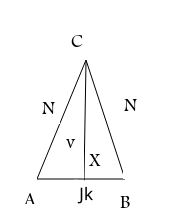
\includegraphics{imagex/trojuholnik.png}
\end{center}

\noindent Teraz si zistíme výšku $v$. Zo zadania vidíme že keď stojí Jožko rozkročený, je o $\frac{1}{20}$ svojej výšky nižší.\\
Jeho výška je 2m, z čoho $\frac{1}{40}$ je $0.1m = 10cm$.
$v$ by teda malo byť $N - 0.1 = 1.042857$.
Na obrázku vidíme pravouhlý trojuholník $XBC$.
Pomocou Pytagorovej vety vypočítame $J_k$:
\[
	(\frac{J_k}{2})^2+v^2 = N^2
\]
Malou úpravou rovnice dostaneme
\[
	(\frac{J_k}{2})^2 = N^2 - v^2
\]
Teraz obe strany rovnice odmocníme, dostaneme
\[
	\frac{J_k}{2} = \sqrt{N^2 - v^2}
\]
Výslednú rovnicu ešte zjednodušíme:
\[
	J_k = \sqrt{N^2 - v^2} \times 2
\]
Teraz môžeme prejsť k samotnému počítaniu:
\begin{center}
\[
	J_k = \sqrt{1.142857^2 - 1.042857^2} \times 2 \approx \sqrt{1.306122 - 1.087551} \times 2 = \sqrt{0.218571} \times 2 \approx 0.467516 \times 2 = 0.935032\ m
\]
\end{center}
\medskip
Vypočítajme Jožkovu rýchlosť $J_R$.\\
Keďže Jožko prejde $J_k$ za $\frac{3}{4}$ sekundy, za $\frac{1}{4}$ sekundy by mal prejsť $\frac{1}{3} \times J_k$, za jednu sekundu by teda mal prejsť $\frac{4}{3} \times J_k \approx 1.246709 m$, z toho vyplýva že $J_R = 1.246709 \frac{m}{s}$
\medskip
\hrule
\end{document}
